\documentclass{beamer}
\usepackage[utf8]{inputenc}
\usepackage[spanish]{babel}
\usepackage{listings}
\usepackage{graphicx}

\renewcommand\lstlistingname{Código}
\renewcommand\lstlistlistingname{Códigos}

\lstset{
    basicstyle=\ttfamily\scriptsize,
    columns=fullflexible,
    keepspaces=true,
    showstringspaces=false,
    commentstyle=\color[gray]{0.4},
    stringstyle=\color[rgb]{0, 0, 0.5},
    frame=single,
    breakatwhitespace=true,
    breaklines=true,
    tabsize=4
}

\AtBeginSection[]{
\begin{frame}
\vfill
\centering
\begin{beamercolorbox}[sep=8pt,center,shadow=true,rounded=true]{title}
\usebeamerfont{title}\insertsectionhead\par
\end{beamercolorbox}
\vfill
\end{frame}
}

\title{
    Memoria de Laboratorio \\
    \large Teledetección
}
\author{Alejandro Domínguez Muñoz}
\institute{Universidad de Sevilla}
\date{Mayo de 2023}

\begin{document}

\frame{\titlepage}

\begin{frame}{Datos de la imagen utilizada}
\begin{columns}
\column{0.5\textwidth}

Zona:
\begin{itemize}
\item Camagüey, Cuba
\item Golfo de México
\item América
\end{itemize}

Fecha:
\begin{itemize}
\item 19-MAY-2023
\end{itemize}

Web:
\begin{itemize}
\item \url{www.eos.com}
\end{itemize}

Sensor:
\begin{itemize}
\item Landsat 8
\end{itemize}

\column{0.5\textwidth}

Dimensiones:
\begin{itemize}
\item 7784 filas
\item 7741 columnas
\end{itemize}

Resolución radiométrica:
\begin{itemize}
\item 16 bits
\end{itemize}

Resolución espacial:
\begin{itemize}
\item 30 m
\end{itemize}

Bandas:
\begin{itemize}
\item 2/BLUE
\item 3/GREEN
\item 4/RED
\item 5/NIR
\item 6/SWIR1
\end{itemize}

\end{columns}
\end{frame}

\section{Imágenes}

\begin{frame}{LAB1: Introducción}
\only<1>{
\begin{figure}[h]
\centering
\includegraphics[height=7cm]{img/1/colorVerdadero.png}
\caption{Composición en color verdadero}
\end{figure}
}
\only<2>{
\begin{figure}[h]
\centering
\includegraphics[height=7cm]{img/1/colorFalso.png}
\caption{Composición en falso color NIR-RED-GREEN}
\end{figure}
}
\end{frame}

\begin{frame}{LAB2: Histograma}
\only<1>{
\begin{figure}[h]
\centering
\includegraphics[width=0.55\textwidth]{img/r.png}
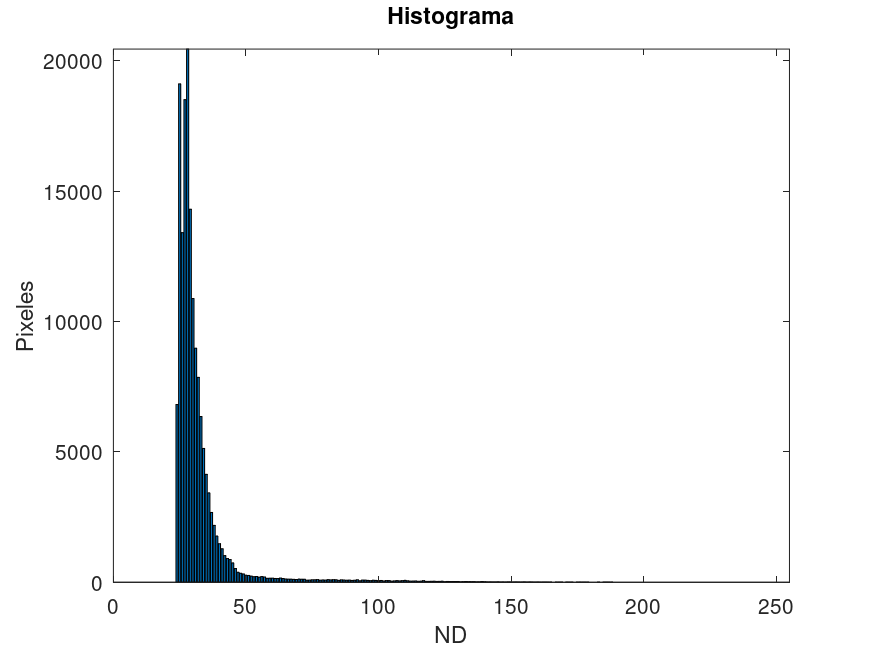
\includegraphics[width=0.4\textwidth]{img/2/r_histo.png}
\caption{Banda RED original}
\end{figure}
}
\only<2>{
\begin{figure}[h]
\centering
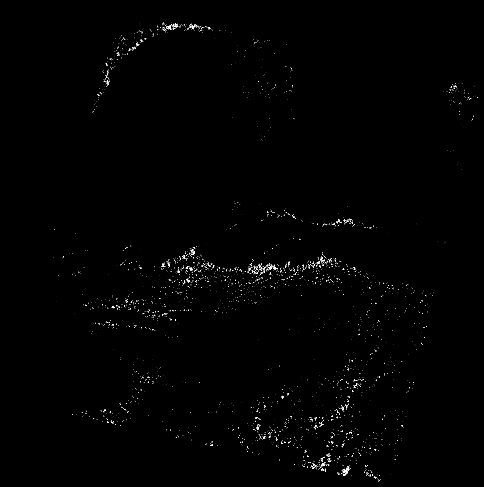
\includegraphics[width=0.55\textwidth]{img/2/imagen_expan_70_130.png}
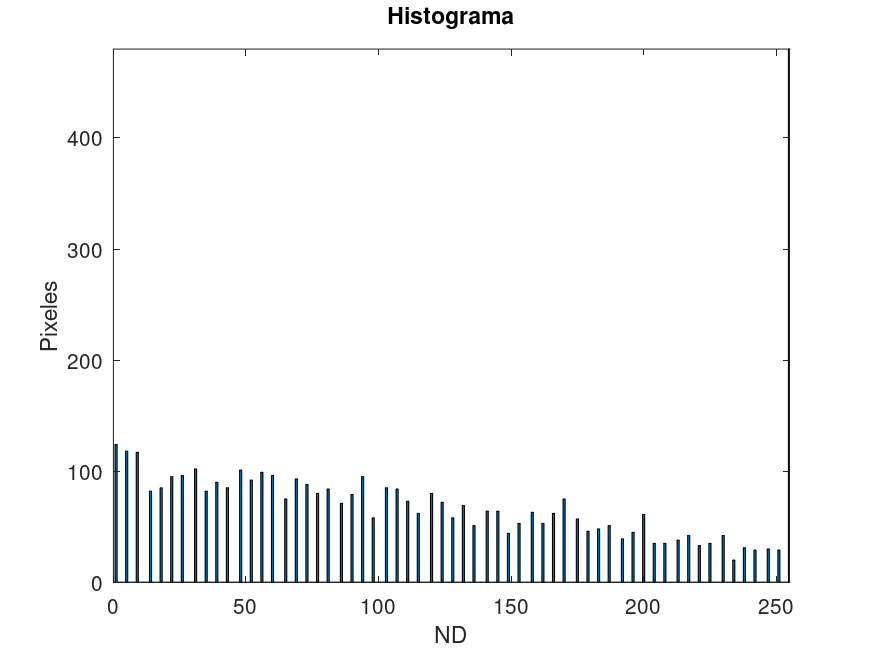
\includegraphics[width=0.4\textwidth]{img/2/imagen_expan_70_130_histo.png}
\caption{Corte de colas dela banda RED: m=70, M=130}
\end{figure}
}
\only<3>{
\begin{figure}[h]
\centering
\includegraphics[width=0.55\textwidth]{img/2/imagen_corte_0.01.png}
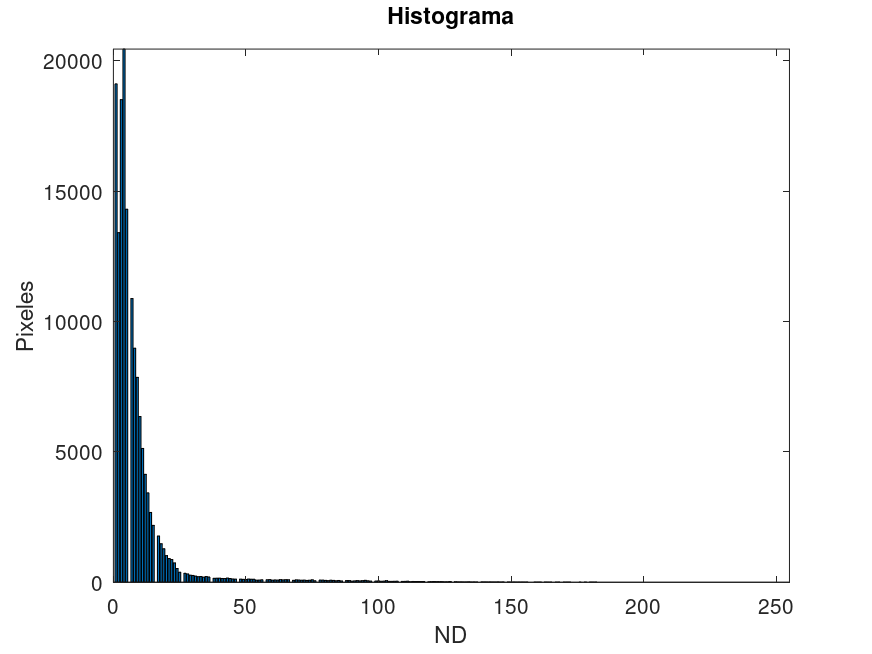
\includegraphics[width=0.4\textwidth]{img/2/imagen_corte_0.01_histo.png}
\caption{Corte de colas al 1\% de la banda RED: m = 25, M = 254}
\end{figure}
}
\only<4>{
\begin{figure}[h]
\centering
\includegraphics[width=0.55\textwidth]{img/2/imagen_ecual.png}
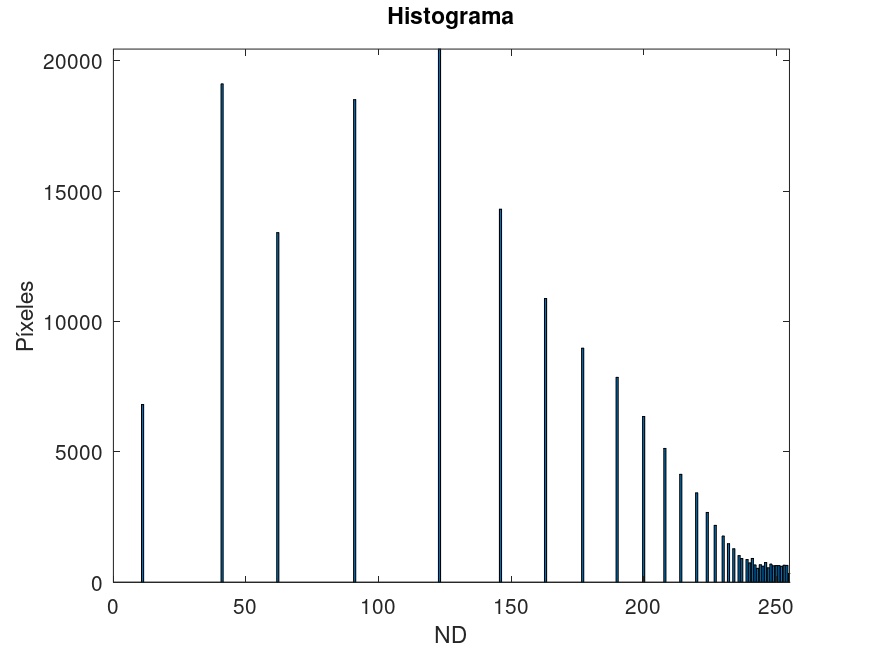
\includegraphics[width=0.4\textwidth]{img/2/imagen_ecual_histo.png}
\caption{Ecualización de la banda RED}
\end{figure}
}
\end{frame}

\begin{frame}{LAB3: Filtrado}
\only<1>{
\begin{columns}
\column{0.5\textwidth}
\begin{figure}[h]
\centering
\includegraphics[width=\textwidth]{img/r.png}
\caption{Banda RED original}
\end{figure}
\column{0.5\textwidth}
\begin{figure}[h]
\centering
\includegraphics[width=\textwidth]{img/3/imagen_mean_filter.png}
\caption{Filtro de media}
\end{figure}
\end{columns}
}
\only<2>{
\begin{columns}
\column{0.5\textwidth}
\begin{figure}[h]
\centering
\includegraphics[width=\textwidth]{img/r.png}
\caption{Banda RED original}
\end{figure}
\column{0.5\textwidth}
\begin{figure}[h]
\centering
\includegraphics[width=\textwidth]{img/3/imagen_mean_filter_normalized.png}
\caption{Filtro de media con normalización de coeficientes}
\end{figure}
\end{columns}
}
\only<3>{
\begin{columns}
\column{0.5\textwidth}
\begin{figure}[h]
\centering
\includegraphics[width=\textwidth]{img/r.png}
\caption{Banda RED original}
\end{figure}
\column{0.5\textwidth}
\begin{figure}[h]
\centering
\includegraphics[width=\textwidth]{img/3/imagen_median_filter.png}
\caption{Filtro de mediana}
\end{figure}
\end{columns}
}
\only<4>{
\begin{columns}
\column{0.5\textwidth}
\begin{figure}[h]
\centering
\includegraphics[width=\textwidth]{img/r.png}
\caption{Banda RED original}
\end{figure}
\column{0.5\textwidth}
\begin{figure}[h]
\centering
\includegraphics[width=\textwidth]{img/3/imagen_median_filter_border.png}
\caption{Filtro de mediana mejorado}
\end{figure}
\end{columns}
}
\only<5>{
\begin{columns}
\column{0.5\textwidth}
\begin{figure}[h]
\centering
\includegraphics[width=\textwidth]{img/r.png}
\caption{Banda RED original}
\end{figure}
\column{0.5\textwidth}
\begin{figure}[h]
\centering
\includegraphics[width=\textwidth]{img/3/imagen_filter_sobel.png}
\caption{Filtro Sobel}
\end{figure}
\end{columns}
}
\end{frame}

\begin{frame}{LAB4: Escalado}
\only<1>{
\begin{columns}
\column{0.5\textwidth}
\begin{figure}[h]
\centering
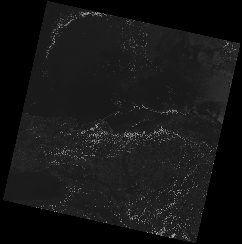
\includegraphics[width=\textwidth]{img/4/imagen_downscaled_x2.png}
\caption{Banda RED original diezmada x2}
\end{figure}
\column{0.5\textwidth}
\begin{figure}[h]
\centering
\includegraphics[width=\textwidth]{img/4/imagen_upscale_bilinear_filter.png}
\caption{Ampliación por interpolación bilineal x2, PSNR = 30.0621}
\end{figure}
\end{columns}
}
\only<2>{
\begin{columns}
\column{0.5\textwidth}
\begin{figure}[h]
\centering
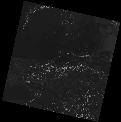
\includegraphics[width=\textwidth]{img/4/imagen_downscaled_x4.png}
\caption{Banda RED original diezmada x4}
\end{figure}
\column{0.5\textwidth}
\begin{figure}[h]
\centering
\includegraphics[width=\textwidth]{img/4/imagen_upscaled_fft.png}
\caption{Ampliación por FFT x4, PSNR = 28.6339}
\end{figure}
\end{columns}
}
\end{frame}

\begin{frame}{LAB5: Color}
\only<1>{
\begin{columns}
\column{0.5\textwidth}
\begin{figure}[h]
\centering
\includegraphics[width=\textwidth]{img/5/imagen_rgb.png}
\caption{Composición en color verdadero}
\end{figure}
\column{0.5\textwidth}
\begin{figure}[h]
\centering
\includegraphics[width=\textwidth]{img/5/imagen_corte_hsv.png}
\caption{Corte en la componente V en dominio HSV}
\end{figure}
\end{columns}
}
\only<2>{
\begin{columns}
\column{0.5\textwidth}
\begin{figure}[h]
\centering
\includegraphics[width=\textwidth]{img/r.png}
\caption{Banda RED original}
\end{figure}
\column{0.5\textwidth}
\begin{figure}[h]
\centering
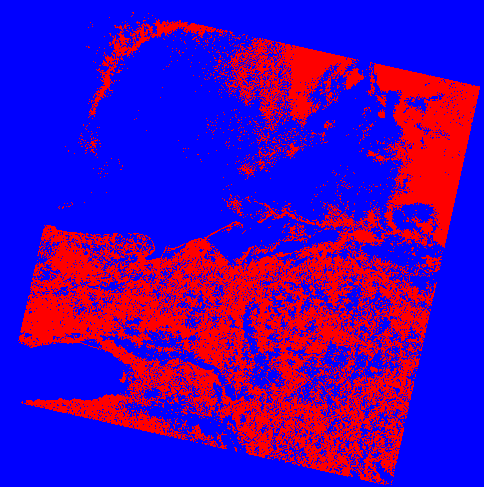
\includegraphics[width=\textwidth]{img/5/imagen_seudo.png}
\caption{Seudocolor, Azul: ND $<$ 30, Rojo: ND $\geq$ 30}
\end{figure}
\end{columns}
}
\only<3>{
\begin{columns}
\column{0.5\textwidth}
\begin{figure}[h]
\centering
\includegraphics[height=2cm]{img/nir.png}
\caption{Banda NIR original}
\end{figure}
\begin{figure}[h]
\centering
\includegraphics[height=2cm]{img/r.png}
\caption{Banda RED original}
\end{figure}
\column{0.5\textwidth}
\begin{figure}[h]
\centering
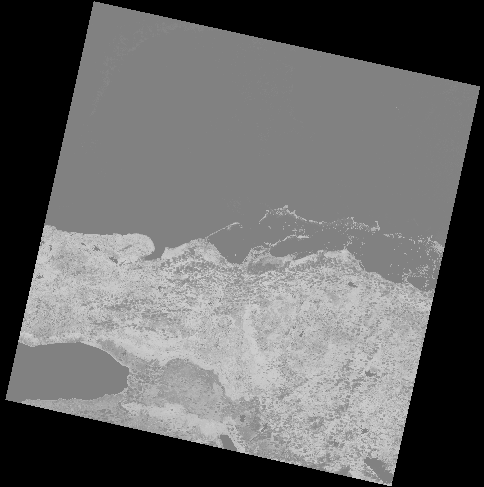
\includegraphics[width=\textwidth]{img/5/imagen_ndvi.png}
\caption{NDVI}
\end{figure}
\end{columns}
}
\only<4>{
\begin{columns}
\column{0.3\textwidth}
\begin{figure}[h]
\centering
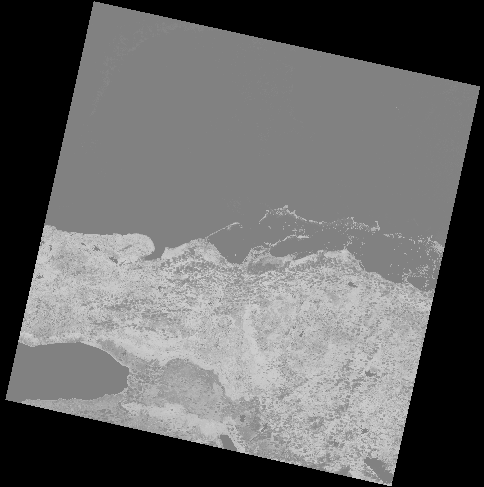
\includegraphics[width=\textwidth]{img/5/imagen_ndvi.png}
\caption{NDVI}
\end{figure}
\column{0.7\textwidth}
\begin{figure}[h]
\centering
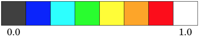
\includegraphics[width=3cm]{chroma_bar.png}
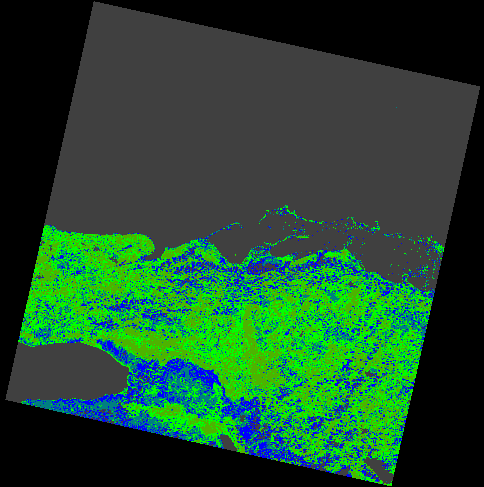
\includegraphics[height=6cm]{img/5/imagen_density.png}
\caption{Density Slicing sobre NDVI}
\end{figure}
\end{columns}
}
\end{frame}

\begin{frame}{LAB6: Clasificación}
\only<1>{
\begin{figure}[h]
\centering
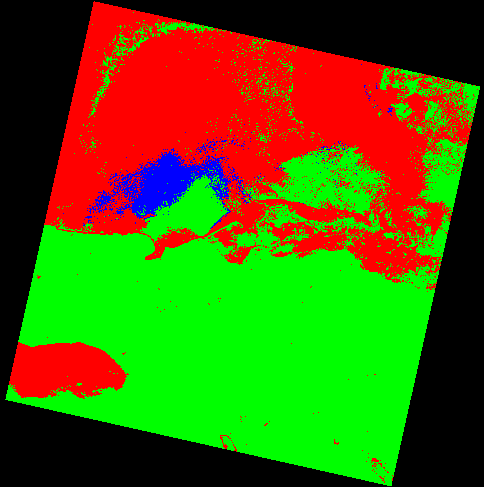
\includegraphics[height=3cm]{img/6/imagen_isodata3.png}
\caption{ISODATA con 3 categorías tras 2 iteraciones}
\end{figure}
Centroides:
\begin{itemize}
\item $C1 = [28.195\ \ \ 38.962\ \ \ 19.697\ \ \ 21.787\ \ \ 23.366]$
\item $C2 = [20.000\ \ \ 22.000\ \ \ 24.594\ \ \ 28.000\ \ \ 38.000]$
\item $C3 = [23.602\ \ \ 25.550\ \ \ 28.128\ \ \ 32.714\ \ \ 40.787]$
\end{itemize}
}
\only<2>{
\begin{figure}[h]
\centering
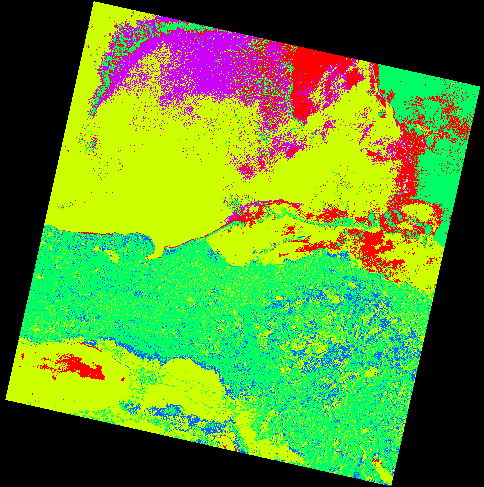
\includegraphics[height=3cm]{img/6/imagen_isodata5.png}
\caption{ISODATA con 5 categorías tras 3 iteraciones}
\end{figure}
Centroides:
\begin{itemize}
\item $C1 = [14.060\ \ \ 16.898\ \ \ 13.899\ \ \ 15.999\ \ \ 19.377]$
\item $C2 = [60.021\ \ \ 82.184\ \ \ 41.288\ \ \ 45.080\ \ \ 47.435]$
\item $C3 = [50.128\ \ \ 83.549\ \ \ 28.800\ \ \ 34.082\ \ \ 35.780]$
\item $C4 = [24.395\ \ \ 26.436\ \ \ 28.608\ \ \ 32.076\ \ \ 41.270]$
\item $C5 = [26.749\ \ \ 28.797\ \ \ 31.245\ \ \ 36.505\ \ \ 43.591]$
\end{itemize}
}
\end{frame}

\section{Código}

\begin{frame}{LAB1: Introducción}
\only<1>{
\lstinputlisting[language=Matlab, caption=facto1.m]{lib/facto1.m}
}
\only<2>{
\lstinputlisting[language=Matlab, caption=facto2.m]{lib/facto2.m}
}
\only<3>{
\lstinputlisting[language=Matlab, caption=sol1.m]{src/sol1.m}
}
\end{frame}

\begin{frame}{LAB2: Histograma}
\only<1>{
\lstinputlisting[language=Matlab, caption=histo.m]{lib/histo.m}
}
\only<2>{
\lstinputlisting[language=Matlab, caption=loadLibs.m]{src/loadLibs.m}
\lstinputlisting[language=Matlab, caption=unloadLibs.m]{src/unloadLibs.m}
}
\only<3>{
\lstinputlisting[language=Matlab, caption=sol2\_1.m]{src/sol2_1.m}
}
\only<4>{
\lstinputlisting[language=Matlab, caption=expan.m]{lib/expan.m}
}
\only<5>{
\lstinputlisting[language=Matlab, caption=sol2\_2.m]{src/sol2_2.m}
}
\only<6>{
\lstinputlisting[language=Matlab, caption=corte.m]{lib/corte.m}
}
\only<7>{
\lstinputlisting[language=Matlab, caption=sol2\_3.m]{src/sol2_3.m}
}
\only<8>{
\lstinputlisting[language=Matlab, caption=ecual.m]{lib/ecual.m}
}
\only<9>{
\lstinputlisting[language=Matlab, caption=sol2\_4.m]{src/sol2_4.m}
}
\end{frame}

\begin{frame}{LAB3: Filtrado}
\only<1>{
\lstinputlisting[language=Matlab, caption=filtro.m]{lib/filtro.m}
}
\only<2>{
\lstinputlisting[language=Matlab, caption=sol3\_1.m]{src/sol3_1.m}
}
\only<3>{
\lstinputlisting[language=Matlab, caption=filtro2.m]{lib/filtro2.m}
}
\only<4>{
\lstinputlisting[language=Matlab, caption=sol3\_2.m]{src/sol3_2.m}
}
\only<5>{
\lstinputlisting[language=Matlab, caption=filtro2.m]{lib/filtro2.m}
}
\only<6>{
\lstinputlisting[language=Matlab, caption=sol3\_2.m]{src/sol3_2.m}
}
\only<7>{
\lstinputlisting[language=Matlab, caption=filtroMediana.m]{lib/filtroMediana.m}
}
\only<8>{
\lstinputlisting[language=Matlab, caption=sol3\_3.m]{src/sol3_3.m}
}
\only<9>{
\lstinputlisting[language=Matlab, caption=filtroMedianaBorde.m]{lib/filtroMedianaBorde.m}
}
\only<10>{
\lstinputlisting[language=Matlab, caption=sol3\_4.m]{src/sol3_4.m}
}
\only<11>{
\lstinputlisting[language=Matlab, caption=filtroSobel.m]{lib/filtroSobel.m}
}
\only<12>{
\lstinputlisting[language=Matlab, caption=sol3\_5.m]{src/sol3_5.m}
}
\end{frame}

\begin{frame}{LAB4: Escalado}
\only<1>{
\lstinputlisting[language=Matlab, caption=diezmado.m]{lib/diezmado.m}
}
\only<2>{
\lstinputlisting[language=Matlab, caption=sol4\_1.m]{src/sol4_1.m}
}
\only<3>{
\lstinputlisting[language=Matlab, caption=amplia.m]{lib/amplia.m}
}
\only<4>{
\lstinputlisting[language=Matlab, caption=sol4\_2.m]{src/sol4_2.m}
}
\only<5>{
\lstinputlisting[language=Matlab, caption=mostrarFFT.m]{lib/mostrarFFT.m}
}
\only<6>{
\lstinputlisting[language=Matlab, caption=sol4\_3.m]{src/sol4_3.m}
}
\only<7>{
\lstinputlisting[language=Matlab, caption=ampliafft.m]{lib/ampliafft.m}
}
\only<8>{
\lstinputlisting[language=Matlab, caption=sol4\_4.m]{src/sol4_4.m}
}
\end{frame}

\begin{frame}{LAB5: Color}
\only<1>{
\lstinputlisting[language=Matlab, caption=falso.m]{lib/falso.m}
}
\only<2>{
\lstinputlisting[language=Matlab, caption=sol5\_1.m]{src/sol5_1.m}
}
\only<3>{
\lstinputlisting[language=Matlab, caption=cortehsv.m]{lib/cortehsv.m}
}
\only<4>{
\lstinputlisting[language=Matlab, caption=sol5\_2.m]{src/sol5_2.m}
}
\only<5>{
\lstinputlisting[language=Matlab, caption=seudo.m]{lib/seudo.m}
}
\only<6>{
\lstinputlisting[language=Matlab, caption=sol5\_3.m]{src/sol5_3.m}
}
\only<7>{
\lstinputlisting[language=Matlab, caption=ndvi.m]{lib/ndvi.m}
}
\only<8>{
\lstinputlisting[language=Matlab, caption=sol5\_4.m]{src/sol5_4.m}
}
\only<9>{
\lstinputlisting[language=Matlab, caption=densi.m]{lib/densi.m}
}
\only<10>{
\lstinputlisting[language=Matlab, caption=sol5\_5.m]{src/sol5_5.m}
}
\end{frame}

\begin{frame}{LAB6: Clasificación}
\only<1>{
\lstinputlisting[
    language=Matlab,
    caption={isodata.m (Preparación)},
    lastline=16
]{lib/isodata.m}
}
\only<2>{
\lstinputlisting[
    language=Matlab,
    caption={isodata.m (Iteraciones)},
    firstline=18,
    lastline=40,
    basicstyle=\ttfamily\tiny
]{lib/isodata.m}
}
\only<3>{
\lstinputlisting[
    language=Matlab,
    caption={isodata.m (Presentación)},
    firstline=42
]{lib/isodata.m}
}
\only<4>{
\lstinputlisting[
    language=Matlab,
    caption=sol6.m,
    basicstyle=\ttfamily\tiny
]{src/sol6.m}
}
\end{frame}

\end{document}